\chapter{自动机状态转移图}

%%  接受{$\mathcal{L}$}=0*10*的自动机{\cite[fig 5-4]{book1}}

\begin{figure}[!htbp]
    \centering
    \begin{subfigure}[b]{0.35\textwidth}
        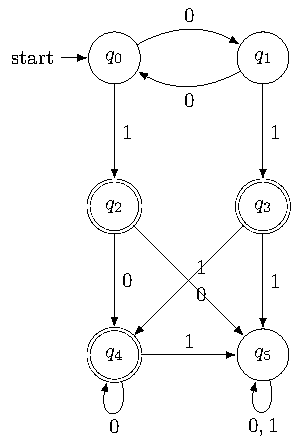
\includegraphics[width=\textwidth]{automaton_4_0}
        \caption{}
        \label{fig:DFA4_0}
    \end{subfigure}
    ~
    \begin{subfigure}[b]{0.35\textwidth}
        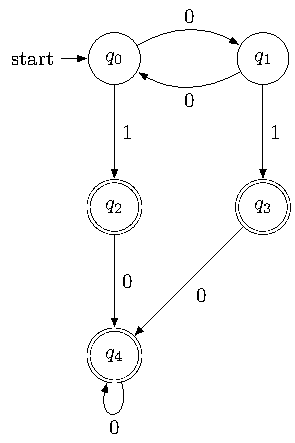
\includegraphics[width=\textwidth]{automaton_4_1}
        \caption{}
        \label{fig:DFA4_1}
    \end{subfigure}
    \\
    \begin{subfigure}[b]{0.35\textwidth}
        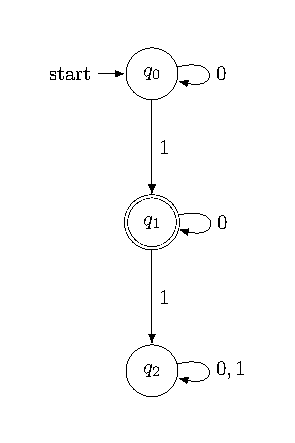
\includegraphics[width=\textwidth]{automaton_4_2}
        \caption{}
        \label{fig:DFA4_2}
    \end{subfigure}
    ~
    \begin{subfigure}[b]{0.35\textwidth}
        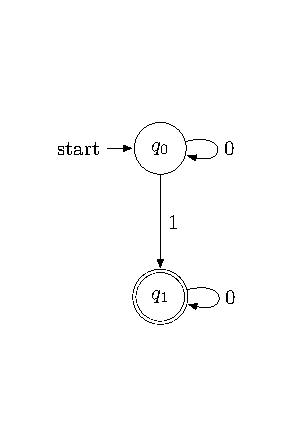
\includegraphics[width=\textwidth]{automaton_4_3}
        \caption{}
        \label{fig:DFA4_3}
    \end{subfigure}
    \caption{(a)接受{$\mathcal{L}$}=0*10*的自动机{\cite[fig 5-4]{book1}};  (b) 图(a)去除非 “final-reachable” 状态 {$q_5$}; (c) 与图(a) 的 $DFA$ 同构的含有陷阱状态的最小 $DFA$ ;(d) 与图(a) 的 $DFA$ 同构的不含陷阱状态的最小 $DFA$。}
    \label{fig:DFA4}
\end{figure}

如图\ref{fig:DFA4}为一个完全自动机


\begin{figure}[!htbp]
    \centering
    \begin{subfigure}[b]{0.35\textwidth}
      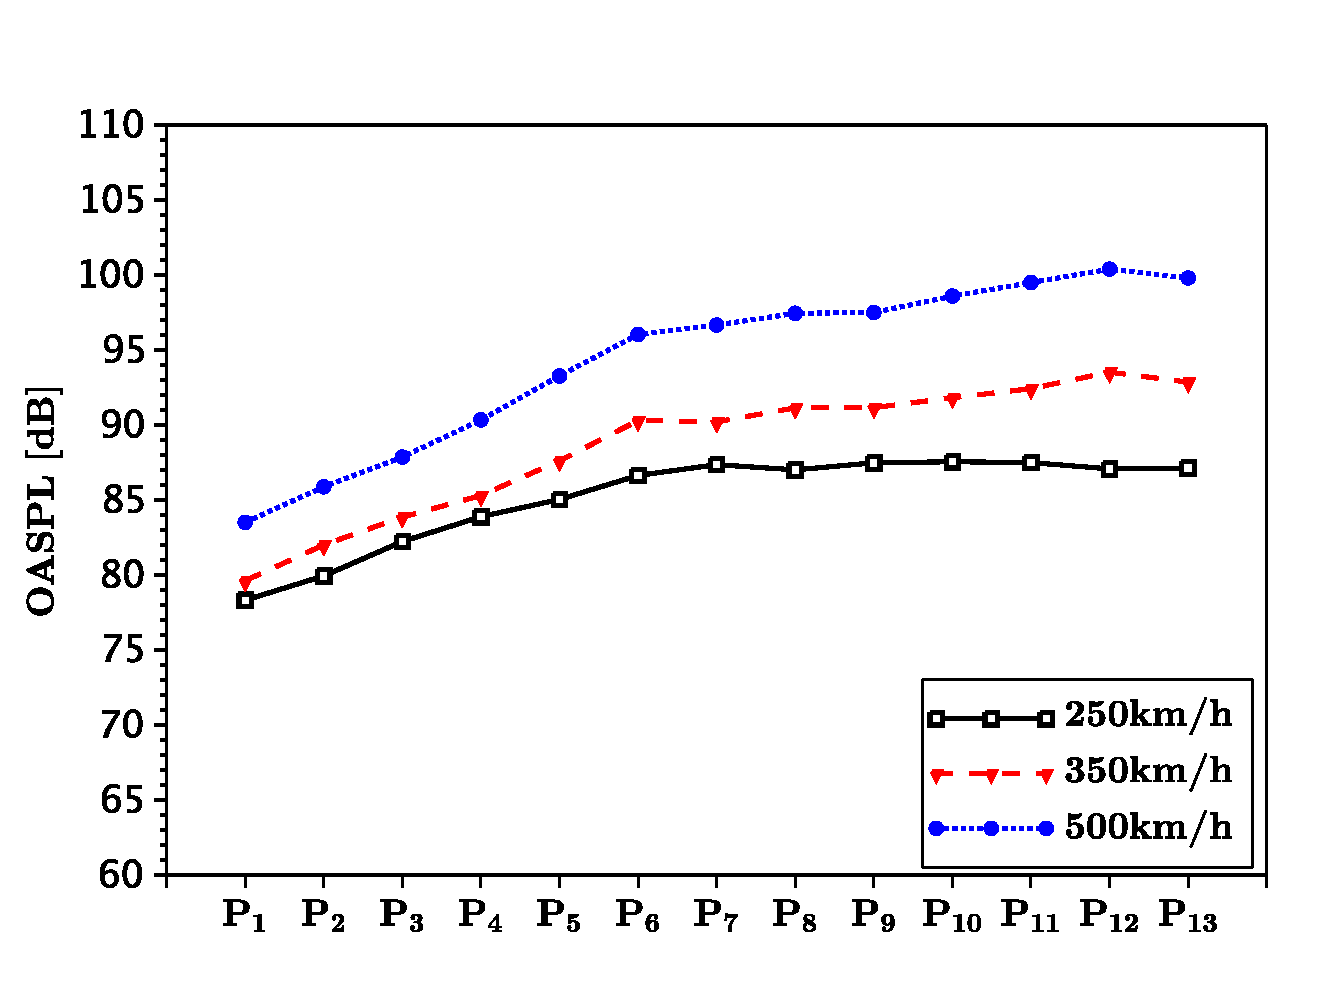
\includegraphics[width=\textwidth]{oaspl_a}
      \caption{}
      \label{fig:oaspl_a}
    \end{subfigure}%
    ~% add desired spacing
    \begin{subfigure}[b]{0.35\textwidth}
      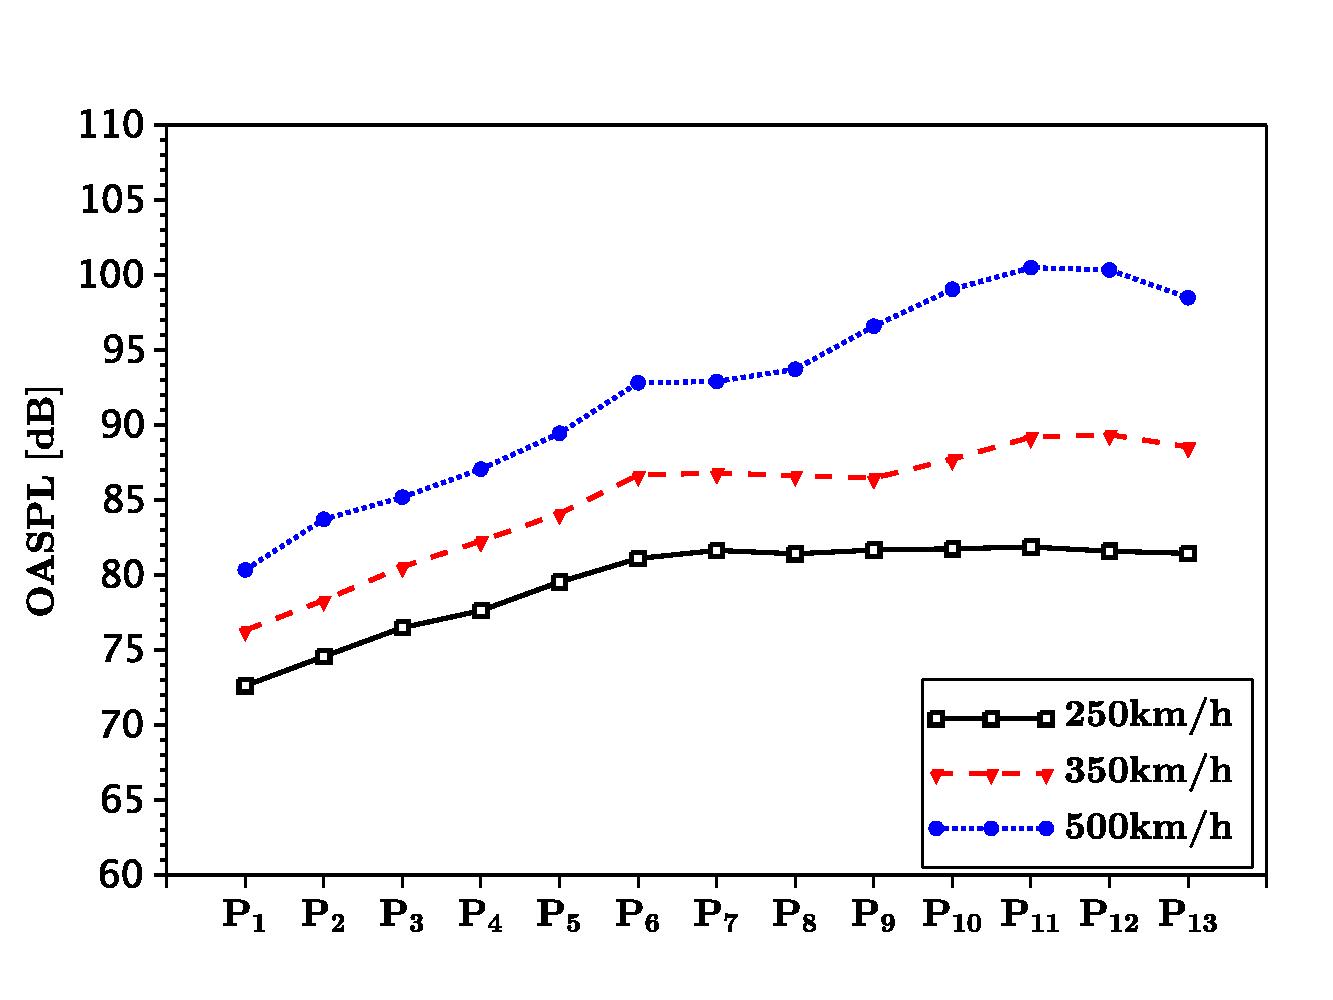
\includegraphics[width=\textwidth]{oaspl_b}
      \caption{}
      \label{fig:oaspl_b}
    \end{subfigure}
    \\% line break
    \begin{subfigure}[b]{0.35\textwidth}
      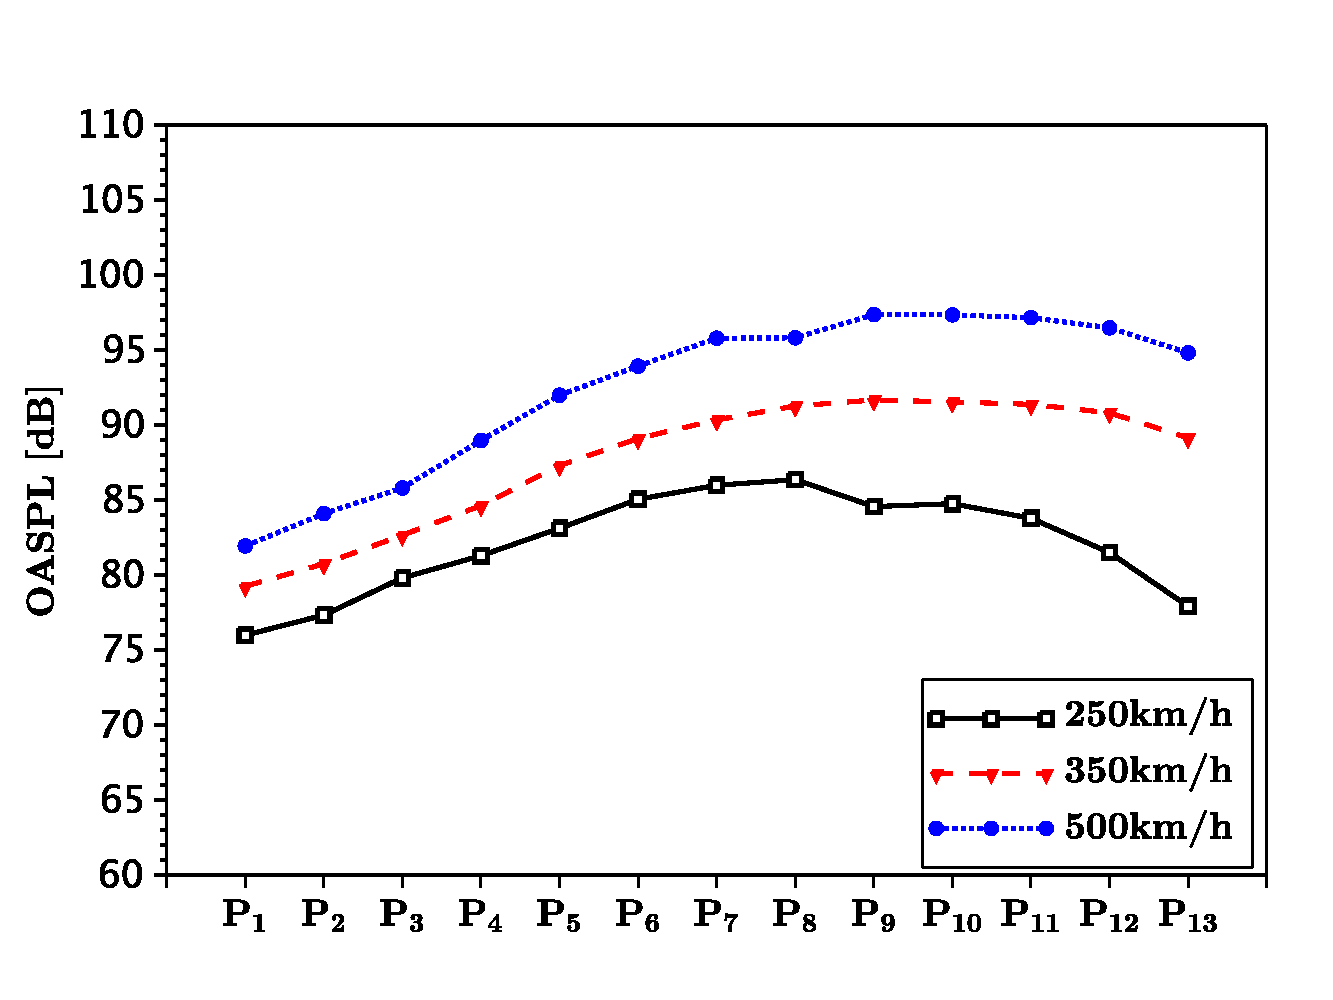
\includegraphics[width=\textwidth]{oaspl_c}
      \caption{}
      \label{fig:oaspl_c}
    \end{subfigure}%
    ~% add desired spacing
    \begin{subfigure}[b]{0.35\textwidth}
      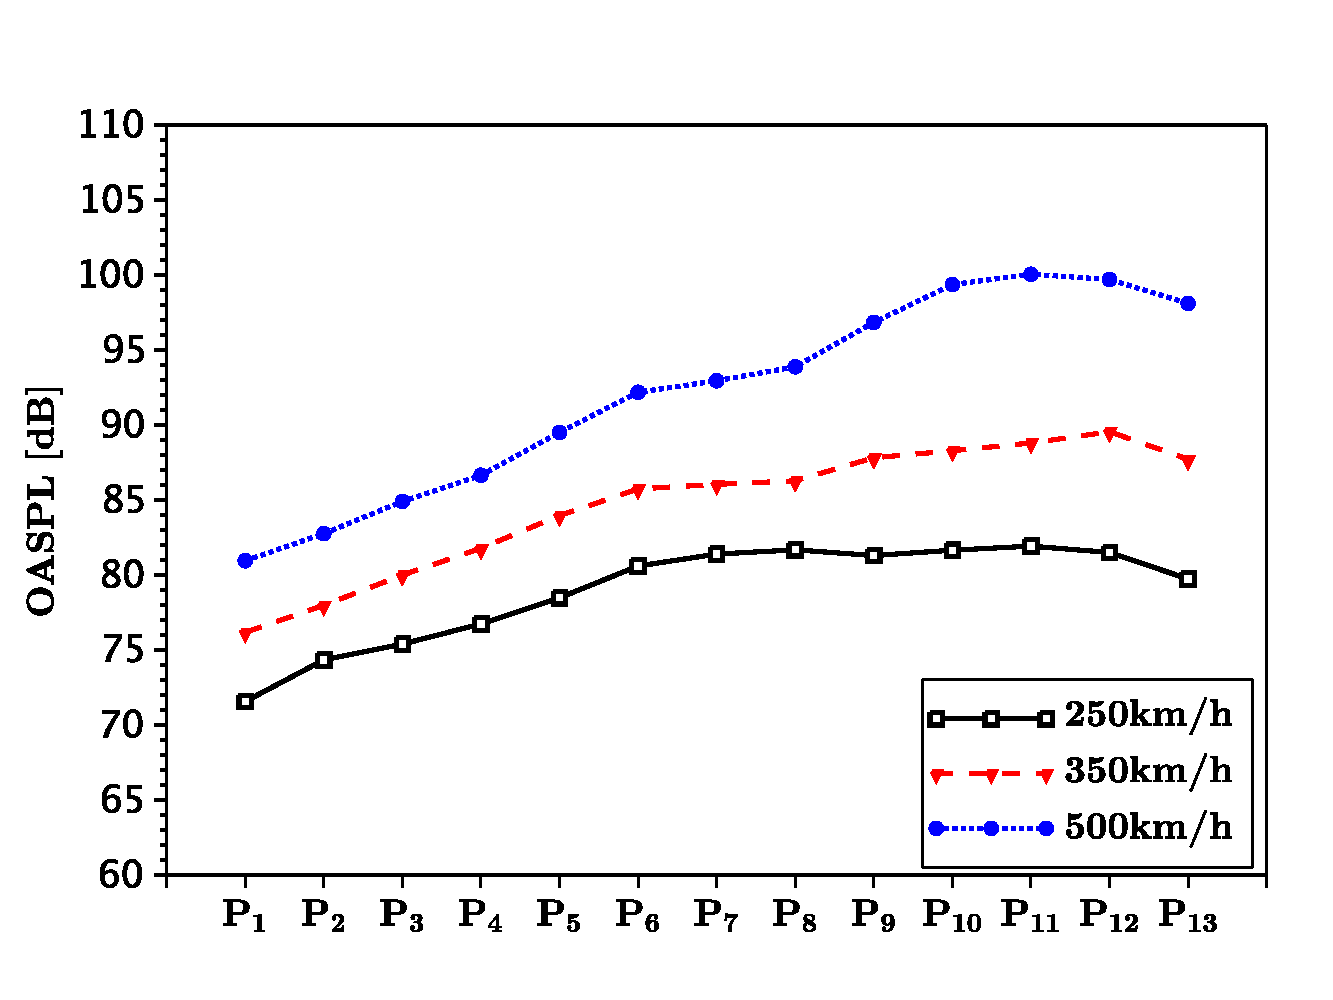
\includegraphics[width=\textwidth]{oaspl_d}
      \caption{}
      \label{fig:oaspl_d}
    \end{subfigure}
    \bicaption{总声压级。(a) 这是子图说明信息,(b) 这是子图说明信息,(c) 这是子图说明信息,(d) 这是子图说明信息。}{OASPL.(a) This is the explanation of subfig, (b) This is the explanation of subfig, (c) This is the explanation of subfig, (d) This is the explanation of subfig.}
    \label{fig:oaspl}
\end{figure}